\subsection{Networks and their proprieties}
A network, mathematically speaking, is defined as a pair of sets $(V,\ E)$, where elements of $V$ are called \textbf{vertices} and $E$ is a set of pairs of vertices, called \textbf{edges}. We also call the vertices \textbf{nodes} and the edges \textbf{links}. With this structure we can describe a set of points ($V$), that can represent some data, and how they are connected each other, through the links.
\begin{figure}[h]
    \centering
    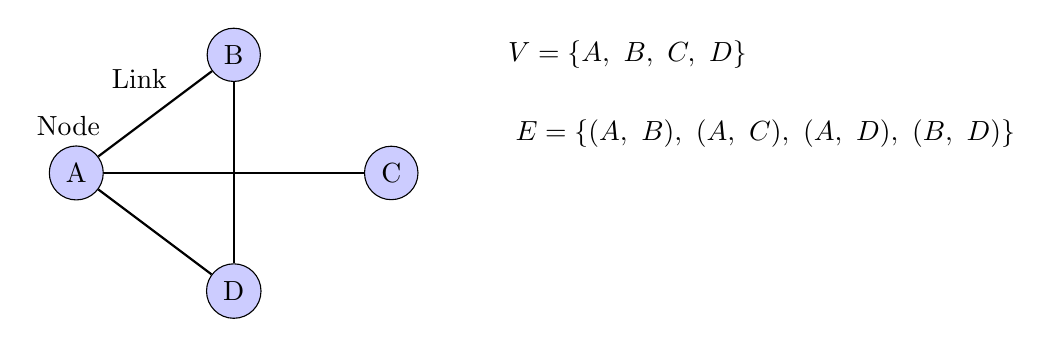
\begin{tikzpicture}
        \node[circle, draw, fill=blue!20] (A) at (0,0) {A};
        \node[circle, draw, fill=blue!20] (B) at (2,1.5) {B};
        \node[circle, draw, fill=blue!20] (C) at (4,0) {C};
        \node[circle, draw, fill=blue!20] (D) at (2,-1.5) {D};
        \node at (-0.1,.6) {Node};
        
        \draw[ thick] (A) -- (B);
        \draw[ thick] (A) -- (C);
        \draw[ thick] (A) -- (D);
        \draw[ thick] (B) -- (D);
        \node at (.8,1.2)  {Link};

        \node at (7,1.5)  {$V=\{A,\ B,\ C,\ D\}$};
        \node at (8.75,0.5)  {$E=\{(A,\ B),\ (A,\ C),\ (A,\ D),\ (B,\ D)\}$};
    \end{tikzpicture}
    \label{Fig:General Network}
    \caption{Pictorial representation of a network: each point is a node and each line connecting nodes is a link.}
\end{figure}  

Network theory can easily be applied to the Ising model in order to describe the lattice structure: each node can represent an atom and each link the possible interactions between neighbors. In this way we also manage to use more general structures, other than square, triangular and hexagonal lattices, that can be then studied numerically. Furthermore, this theory allows us to study the proprieties of a network by measuring some quantities that can be then used to analyze its structure.
\subsubsection{Topologies of a network}
As we already said, using networks to describe the lattice allows us to easily study, by numerical methods, different types of topologies in different dimensions: starting from $2D$ lattices with different structures, square, triangular, hexagonal lattices, to $3D$ lattices to Erdős–Rényi graphs and so on. Let's spend some time analyzing the graph that we used.

Lattices are regular networks that periodically repeat a basic structure: square lattices are made by the repetition of 4 nodes connected together into a square, triangular by 3 nodes to form a triangle and lastly hexagonal are made by groups of 6 nodes forming hexagons. These structures can also be created in 3 dimensions or higher.

Herdos Renyl graphs are networks made up by a fixed number of nodes $N$ and are characterized by a probability $p$: this is the probability that a pair of nodes is connected by a link. In this way the number of links connected to a node (degree of the node) follows the binomial distribution.

Lastly, we used some more specific networks: we call \emph{broken lattices} lattices from which we removed a fraction of vertices (and their edges), and \emph{more than nearest neighbors} lattices in which we connected each node to the neighbors of its neighbors.


\subsubsection{Measuring proprieties of networks}
To end our introduction on networks, we will now illustrate the main quantities that we aim to measure in our simulation of the Ising model.
\begin{itemize}
    \item \textbf{Network density}: this parameter measure how many links are present in a network compared to the maximum number of links possible given the nodes, it is defined as:
    \begin{equation}
        d=\frac{2m}{n(n-1)},\label{density}
    \end{equation}
    where $m$ is the number of edges and $n$ the number of nodes, $\frac{n(n-1)}{2}$ is the maximum number of edges given $n$ nodes.
    \item \textbf{Diameter}: this measures the minimum number of links connecting the two farthest nodes of a connected graph (if every point can be reached moving along the graph starting from every other point), it is defined as:
    \begin{equation}
        D=\max_{i,j} D_{i,j},\label{diameter}
    \end{equation}
    where $D_{ij}$ is the geodesic distance between node $i$ and $j$, which is the number of links of the shortest path connecting $i$ to $j$.
    \item \textbf{Betweenness centrality}: for every node we can measure how the network changes removing 1 node, this is done by this quantity defined by:
    \begin{equation}
        \label{Betweenness centrality}
        B_i=\sum_{j,k\neq i}\frac{N_{jik}}{N_{jk}},
    \end{equation}
    where $N_{jik}$ is the number of the shortest path starting form the node $j$, passing for the node $i$ and ending in the node $k$ and $N_{jk}$ are the shortest path from the node $j$ to node $k$, in this way we measure the fraction of the shortest paths that would be broken by removing the $i$-th node.
    \item \textbf{Node connectivity}: this quantifies the minimum number of nodes needed to be removed in order to disconnect the graph or make it trivial.
\end{itemize}
Note that all the networks described in the previous section have precise proprieties, therefore we won't measure these quantities for the lattice networks, but we will study the networks emerging from the Ising dynamic.

Discussing these proprieties we introduced the concept of a connected graph, for which every pair of point can be connected moving along the network, however this implies that there can be also network that are disconnected. This kind of networks are composed by at least two connected subnetworks: it can be interesting to study the proprieties of these connected components, for this reason we use the \textbf{number of connected components} and the \textbf{giant component}, which is the largest connected component. The giant component can then be used to study the behavior of those quantities, as the betweenness centrality, that cannot be defined on disconnected networks. 
